% Created by tikzDevice version 0.12.6 on 2024-02-18 17:33:14
% !TEX encoding = UTF-8 Unicode
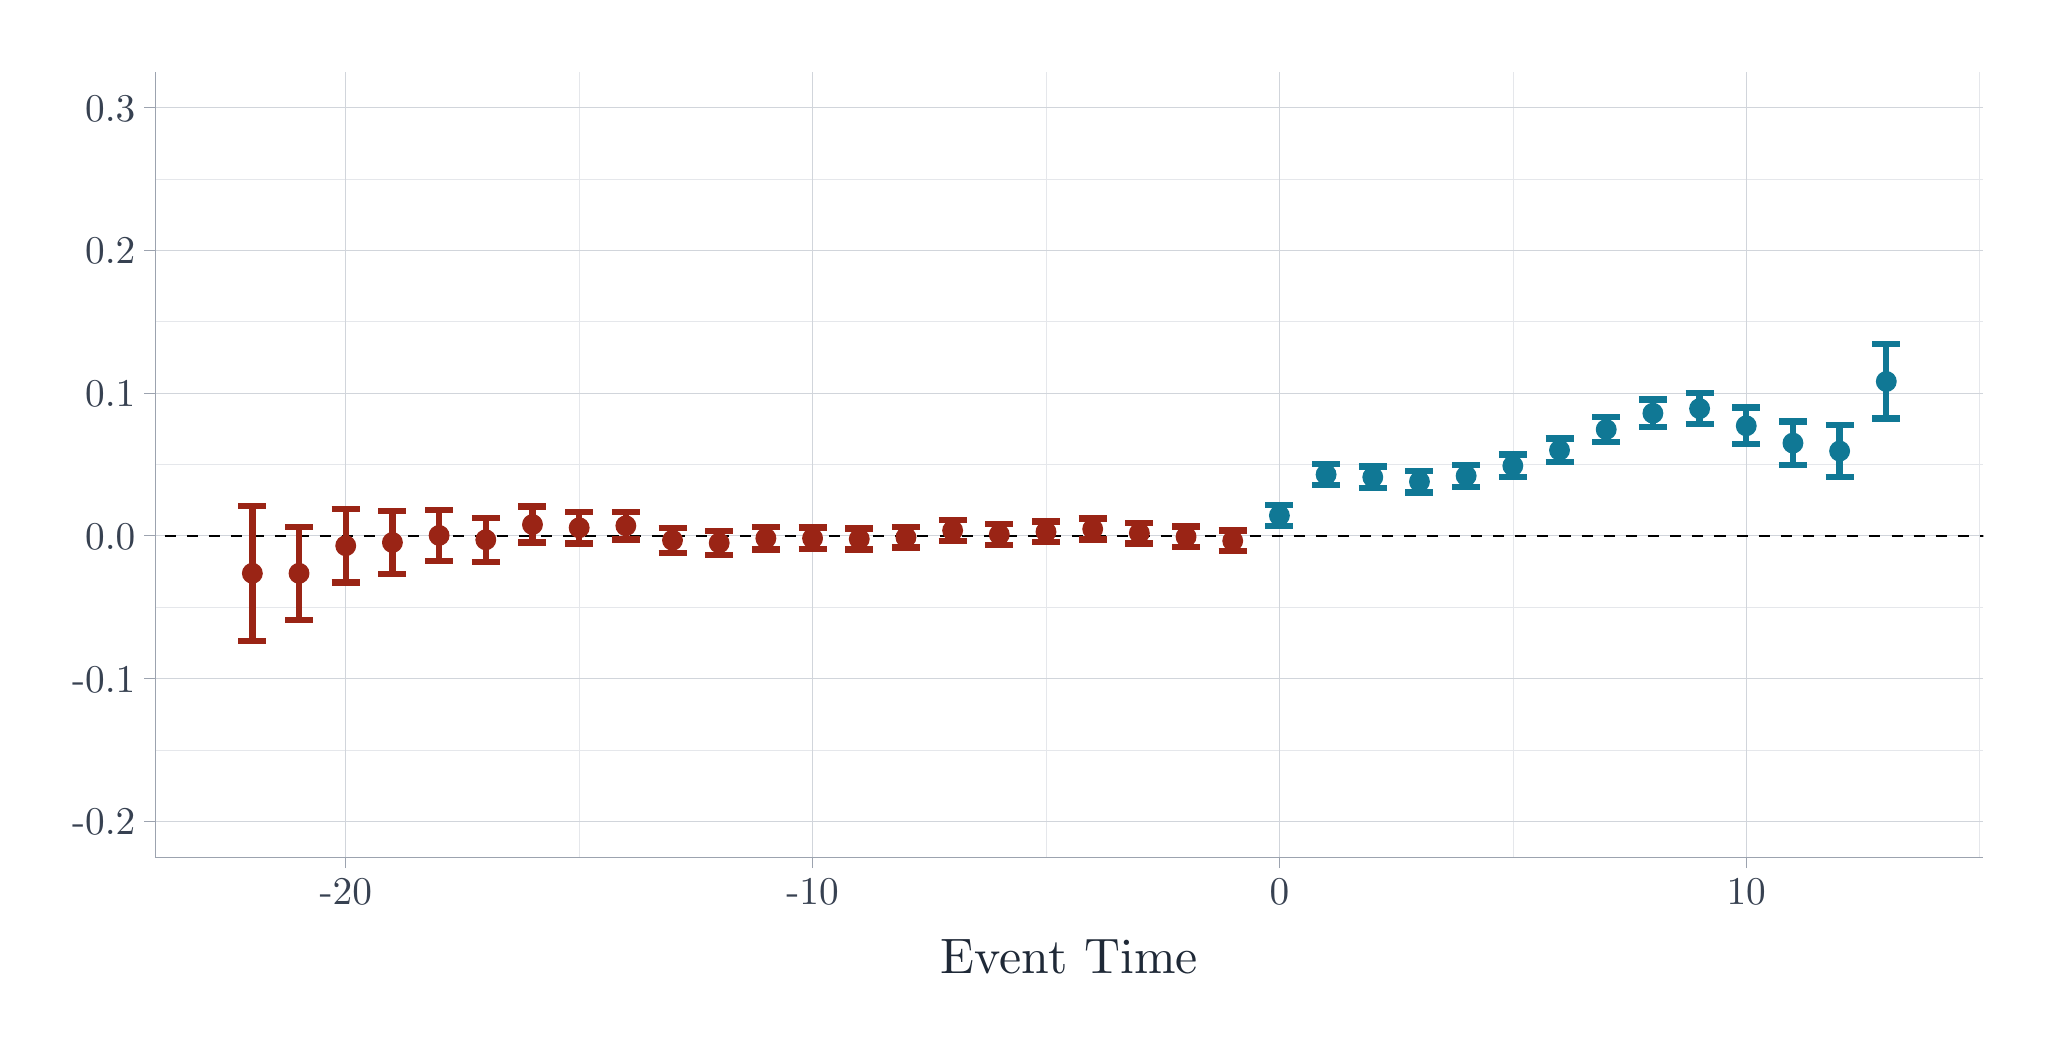
\begin{tikzpicture}[x=1pt,y=1pt]
\definecolor{fillColor}{RGB}{255,255,255}
\path[use as bounding box,fill=fillColor] (0,0) rectangle (722.70,361.35);
\begin{scope}
\path[clip] (  0.00,  0.00) rectangle (722.70,361.35);
\definecolor{drawColor}{RGB}{255,255,255}

\path[draw=drawColor,line width= 0.8pt,line join=round,line cap=round,fill=fillColor] (  0.00,  0.00) rectangle (722.70,361.35);
\end{scope}
\begin{scope}
\path[clip] ( 46.10, 61.65) rectangle (706.70,345.35);
\definecolor{drawColor}{RGB}{255,255,255}
\definecolor{fillColor}{RGB}{255,255,255}

\path[draw=drawColor,line width= 0.8pt,line join=round,line cap=round,fill=fillColor] ( 46.10, 61.65) rectangle (706.70,345.35);
\definecolor{drawColor}{RGB}{229,231,235}

\path[draw=drawColor,line width= 0.2pt,line join=round] ( 46.10,100.34) --
	(706.70,100.34);

\path[draw=drawColor,line width= 0.2pt,line join=round] ( 46.10,151.92) --
	(706.70,151.92);

\path[draw=drawColor,line width= 0.2pt,line join=round] ( 46.10,203.50) --
	(706.70,203.50);

\path[draw=drawColor,line width= 0.2pt,line join=round] ( 46.10,255.08) --
	(706.70,255.08);

\path[draw=drawColor,line width= 0.2pt,line join=round] ( 46.10,306.66) --
	(706.70,306.66);

\path[draw=drawColor,line width= 0.2pt,line join=round] (199.28, 61.65) --
	(199.28,345.35);

\path[draw=drawColor,line width= 0.2pt,line join=round] (367.97, 61.65) --
	(367.97,345.35);

\path[draw=drawColor,line width= 0.2pt,line join=round] (536.66, 61.65) --
	(536.66,345.35);

\path[draw=drawColor,line width= 0.2pt,line join=round] (705.35, 61.65) --
	(705.35,345.35);
\definecolor{drawColor}{RGB}{209,213,219}

\path[draw=drawColor,line width= 0.4pt,line join=round] ( 46.10, 74.55) --
	(706.70, 74.55);

\path[draw=drawColor,line width= 0.4pt,line join=round] ( 46.10,126.13) --
	(706.70,126.13);

\path[draw=drawColor,line width= 0.4pt,line join=round] ( 46.10,177.71) --
	(706.70,177.71);

\path[draw=drawColor,line width= 0.4pt,line join=round] ( 46.10,229.29) --
	(706.70,229.29);

\path[draw=drawColor,line width= 0.4pt,line join=round] ( 46.10,280.87) --
	(706.70,280.87);

\path[draw=drawColor,line width= 0.4pt,line join=round] ( 46.10,332.45) --
	(706.70,332.45);

\path[draw=drawColor,line width= 0.4pt,line join=round] (114.93, 61.65) --
	(114.93,345.35);

\path[draw=drawColor,line width= 0.4pt,line join=round] (283.62, 61.65) --
	(283.62,345.35);

\path[draw=drawColor,line width= 0.4pt,line join=round] (452.31, 61.65) --
	(452.31,345.35);

\path[draw=drawColor,line width= 0.4pt,line join=round] (621.00, 61.65) --
	(621.00,345.35);
\definecolor{drawColor}{RGB}{0,0,0}

\path[draw=drawColor,line width= 0.9pt,dash pattern=on 4pt off 4pt ,line join=round] (-614.49,177.71) -- (1367.30,177.71);
\definecolor{drawColor}{RGB}{154,36,21}
\definecolor{fillColor}{RGB}{154,36,21}

\path[draw=drawColor,line width= 0.4pt,line join=round,line cap=round,fill=fillColor] ( 81.19,164.18) circle (  3.57);

\path[draw=drawColor,line width= 0.4pt,line join=round,line cap=round,fill=fillColor] ( 98.06,164.18) circle (  3.57);

\path[draw=drawColor,line width= 0.4pt,line join=round,line cap=round,fill=fillColor] (114.93,174.15) circle (  3.57);

\path[draw=drawColor,line width= 0.4pt,line join=round,line cap=round,fill=fillColor] (131.80,175.32) circle (  3.57);

\path[draw=drawColor,line width= 0.4pt,line join=round,line cap=round,fill=fillColor] (148.67,177.87) circle (  3.57);

\path[draw=drawColor,line width= 0.4pt,line join=round,line cap=round,fill=fillColor] (165.54,176.30) circle (  3.57);

\path[draw=drawColor,line width= 0.4pt,line join=round,line cap=round,fill=fillColor] (182.41,181.80) circle (  3.57);

\path[draw=drawColor,line width= 0.4pt,line join=round,line cap=round,fill=fillColor] (199.28,180.64) circle (  3.57);

\path[draw=drawColor,line width= 0.4pt,line join=round,line cap=round,fill=fillColor] (216.15,181.36) circle (  3.57);

\path[draw=drawColor,line width= 0.4pt,line join=round,line cap=round,fill=fillColor] (233.01,176.14) circle (  3.57);

\path[draw=drawColor,line width= 0.4pt,line join=round,line cap=round,fill=fillColor] (249.88,175.13) circle (  3.57);

\path[draw=drawColor,line width= 0.4pt,line join=round,line cap=round,fill=fillColor] (266.75,176.85) circle (  3.57);

\path[draw=drawColor,line width= 0.4pt,line join=round,line cap=round,fill=fillColor] (283.62,176.84) circle (  3.57);

\path[draw=drawColor,line width= 0.4pt,line join=round,line cap=round,fill=fillColor] (300.49,176.58) circle (  3.57);

\path[draw=drawColor,line width= 0.4pt,line join=round,line cap=round,fill=fillColor] (317.36,177.18) circle (  3.57);

\path[draw=drawColor,line width= 0.4pt,line join=round,line cap=round,fill=fillColor] (334.23,179.68) circle (  3.57);

\path[draw=drawColor,line width= 0.4pt,line join=round,line cap=round,fill=fillColor] (351.10,178.18) circle (  3.57);

\path[draw=drawColor,line width= 0.4pt,line join=round,line cap=round,fill=fillColor] (367.97,179.19) circle (  3.57);

\path[draw=drawColor,line width= 0.4pt,line join=round,line cap=round,fill=fillColor] (384.84,180.19) circle (  3.57);

\path[draw=drawColor,line width= 0.4pt,line join=round,line cap=round,fill=fillColor] (401.71,178.70) circle (  3.57);

\path[draw=drawColor,line width= 0.4pt,line join=round,line cap=round,fill=fillColor] (418.58,177.38) circle (  3.57);

\path[draw=drawColor,line width= 0.4pt,line join=round,line cap=round,fill=fillColor] (435.44,175.90) circle (  3.57);
\definecolor{drawColor}{RGB}{16,120,149}
\definecolor{fillColor}{RGB}{16,120,149}

\path[draw=drawColor,line width= 0.4pt,line join=round,line cap=round,fill=fillColor] (452.31,185.05) circle (  3.57);

\path[draw=drawColor,line width= 0.4pt,line join=round,line cap=round,fill=fillColor] (469.18,199.87) circle (  3.57);

\path[draw=drawColor,line width= 0.4pt,line join=round,line cap=round,fill=fillColor] (486.05,198.93) circle (  3.57);

\path[draw=drawColor,line width= 0.4pt,line join=round,line cap=round,fill=fillColor] (502.92,197.31) circle (  3.57);

\path[draw=drawColor,line width= 0.4pt,line join=round,line cap=round,fill=fillColor] (519.79,199.39) circle (  3.57);

\path[draw=drawColor,line width= 0.4pt,line join=round,line cap=round,fill=fillColor] (536.66,203.03) circle (  3.57);

\path[draw=drawColor,line width= 0.4pt,line join=round,line cap=round,fill=fillColor] (553.53,208.66) circle (  3.57);

\path[draw=drawColor,line width= 0.4pt,line join=round,line cap=round,fill=fillColor] (570.40,216.15) circle (  3.57);

\path[draw=drawColor,line width= 0.4pt,line join=round,line cap=round,fill=fillColor] (587.27,222.02) circle (  3.57);

\path[draw=drawColor,line width= 0.4pt,line join=round,line cap=round,fill=fillColor] (604.14,223.69) circle (  3.57);

\path[draw=drawColor,line width= 0.4pt,line join=round,line cap=round,fill=fillColor] (621.00,217.48) circle (  3.57);

\path[draw=drawColor,line width= 0.4pt,line join=round,line cap=round,fill=fillColor] (637.87,211.23) circle (  3.57);

\path[draw=drawColor,line width= 0.4pt,line join=round,line cap=round,fill=fillColor] (654.74,208.36) circle (  3.57);

\path[draw=drawColor,line width= 0.4pt,line join=round,line cap=round,fill=fillColor] (671.61,233.50) circle (  3.57);
\definecolor{drawColor}{RGB}{154,36,21}

\path[draw=drawColor,line width= 2.3pt,line join=round] ( 76.13,188.54) --
	( 86.25,188.54);

\path[draw=drawColor,line width= 2.3pt,line join=round] ( 81.19,188.54) --
	( 81.19,139.82);

\path[draw=drawColor,line width= 2.3pt,line join=round] ( 76.13,139.82) --
	( 86.25,139.82);

\path[draw=drawColor,line width= 2.3pt,line join=round] ( 93.00,181.01) --
	(103.12,181.01);

\path[draw=drawColor,line width= 2.3pt,line join=round] ( 98.06,181.01) --
	( 98.06,147.36);

\path[draw=drawColor,line width= 2.3pt,line join=round] ( 93.00,147.36) --
	(103.12,147.36);

\path[draw=drawColor,line width= 2.3pt,line join=round] (109.87,187.49) --
	(119.99,187.49);

\path[draw=drawColor,line width= 2.3pt,line join=round] (114.93,187.49) --
	(114.93,160.81);

\path[draw=drawColor,line width= 2.3pt,line join=round] (109.87,160.81) --
	(119.99,160.81);

\path[draw=drawColor,line width= 2.3pt,line join=round] (126.74,186.77) --
	(136.86,186.77);

\path[draw=drawColor,line width= 2.3pt,line join=round] (131.80,186.77) --
	(131.80,163.86);

\path[draw=drawColor,line width= 2.3pt,line join=round] (126.74,163.86) --
	(136.86,163.86);

\path[draw=drawColor,line width= 2.3pt,line join=round] (143.61,187.04) --
	(153.73,187.04);

\path[draw=drawColor,line width= 2.3pt,line join=round] (148.67,187.04) --
	(148.67,168.69);

\path[draw=drawColor,line width= 2.3pt,line join=round] (143.61,168.69) --
	(153.73,168.69);

\path[draw=drawColor,line width= 2.3pt,line join=round] (160.48,184.28) --
	(170.60,184.28);

\path[draw=drawColor,line width= 2.3pt,line join=round] (165.54,184.28) --
	(165.54,168.33);

\path[draw=drawColor,line width= 2.3pt,line join=round] (160.48,168.33) --
	(170.60,168.33);

\path[draw=drawColor,line width= 2.3pt,line join=round] (177.35,188.31) --
	(187.47,188.31);

\path[draw=drawColor,line width= 2.3pt,line join=round] (182.41,188.31) --
	(182.41,175.29);

\path[draw=drawColor,line width= 2.3pt,line join=round] (177.35,175.29) --
	(187.47,175.29);

\path[draw=drawColor,line width= 2.3pt,line join=round] (194.22,186.35) --
	(204.34,186.35);

\path[draw=drawColor,line width= 2.3pt,line join=round] (199.28,186.35) --
	(199.28,174.93);

\path[draw=drawColor,line width= 2.3pt,line join=round] (194.22,174.93) --
	(204.34,174.93);

\path[draw=drawColor,line width= 2.3pt,line join=round] (211.08,186.38) --
	(221.21,186.38);

\path[draw=drawColor,line width= 2.3pt,line join=round] (216.15,186.38) --
	(216.15,176.34);

\path[draw=drawColor,line width= 2.3pt,line join=round] (211.08,176.34) --
	(221.21,176.34);

\path[draw=drawColor,line width= 2.3pt,line join=round] (227.95,180.65) --
	(238.08,180.65);

\path[draw=drawColor,line width= 2.3pt,line join=round] (233.01,180.65) --
	(233.01,171.63);

\path[draw=drawColor,line width= 2.3pt,line join=round] (227.95,171.63) --
	(238.08,171.63);

\path[draw=drawColor,line width= 2.3pt,line join=round] (244.82,179.38) --
	(254.94,179.38);

\path[draw=drawColor,line width= 2.3pt,line join=round] (249.88,179.38) --
	(249.88,170.88);

\path[draw=drawColor,line width= 2.3pt,line join=round] (244.82,170.88) --
	(254.94,170.88);

\path[draw=drawColor,line width= 2.3pt,line join=round] (261.69,180.92) --
	(271.81,180.92);

\path[draw=drawColor,line width= 2.3pt,line join=round] (266.75,180.92) --
	(266.75,172.77);

\path[draw=drawColor,line width= 2.3pt,line join=round] (261.69,172.77) --
	(271.81,172.77);

\path[draw=drawColor,line width= 2.3pt,line join=round] (278.56,180.73) --
	(288.68,180.73);

\path[draw=drawColor,line width= 2.3pt,line join=round] (283.62,180.73) --
	(283.62,172.95);

\path[draw=drawColor,line width= 2.3pt,line join=round] (278.56,172.95) --
	(288.68,172.95);

\path[draw=drawColor,line width= 2.3pt,line join=round] (295.43,180.31) --
	(305.55,180.31);

\path[draw=drawColor,line width= 2.3pt,line join=round] (300.49,180.31) --
	(300.49,172.84);

\path[draw=drawColor,line width= 2.3pt,line join=round] (295.43,172.84) --
	(305.55,172.84);

\path[draw=drawColor,line width= 2.3pt,line join=round] (312.30,180.92) --
	(322.42,180.92);

\path[draw=drawColor,line width= 2.3pt,line join=round] (317.36,180.92) --
	(317.36,173.45);

\path[draw=drawColor,line width= 2.3pt,line join=round] (312.30,173.45) --
	(322.42,173.45);

\path[draw=drawColor,line width= 2.3pt,line join=round] (329.17,183.42) --
	(339.29,183.42);

\path[draw=drawColor,line width= 2.3pt,line join=round] (334.23,183.42) --
	(334.23,175.95);

\path[draw=drawColor,line width= 2.3pt,line join=round] (329.17,175.95) --
	(339.29,175.95);

\path[draw=drawColor,line width= 2.3pt,line join=round] (346.04,181.91) --
	(356.16,181.91);

\path[draw=drawColor,line width= 2.3pt,line join=round] (351.10,181.91) --
	(351.10,174.44);

\path[draw=drawColor,line width= 2.3pt,line join=round] (346.04,174.44) --
	(356.16,174.44);

\path[draw=drawColor,line width= 2.3pt,line join=round] (362.91,182.93) --
	(373.03,182.93);

\path[draw=drawColor,line width= 2.3pt,line join=round] (367.97,182.93) --
	(367.97,175.45);

\path[draw=drawColor,line width= 2.3pt,line join=round] (362.91,175.45) --
	(373.03,175.45);

\path[draw=drawColor,line width= 2.3pt,line join=round] (379.78,183.93) --
	(389.90,183.93);

\path[draw=drawColor,line width= 2.3pt,line join=round] (384.84,183.93) --
	(384.84,176.46);

\path[draw=drawColor,line width= 2.3pt,line join=round] (379.78,176.46) --
	(389.90,176.46);

\path[draw=drawColor,line width= 2.3pt,line join=round] (396.65,182.44) --
	(406.77,182.44);

\path[draw=drawColor,line width= 2.3pt,line join=round] (401.71,182.44) --
	(401.71,174.97);

\path[draw=drawColor,line width= 2.3pt,line join=round] (396.65,174.97) --
	(406.77,174.97);

\path[draw=drawColor,line width= 2.3pt,line join=round] (413.51,181.12) --
	(423.64,181.12);

\path[draw=drawColor,line width= 2.3pt,line join=round] (418.58,181.12) --
	(418.58,173.65);

\path[draw=drawColor,line width= 2.3pt,line join=round] (413.51,173.65) --
	(423.64,173.65);

\path[draw=drawColor,line width= 2.3pt,line join=round] (430.38,179.63) --
	(440.50,179.63);

\path[draw=drawColor,line width= 2.3pt,line join=round] (435.44,179.63) --
	(435.44,172.16);

\path[draw=drawColor,line width= 2.3pt,line join=round] (430.38,172.16) --
	(440.50,172.16);
\definecolor{drawColor}{RGB}{16,120,149}

\path[draw=drawColor,line width= 2.3pt,line join=round] (447.25,188.79) --
	(457.37,188.79);

\path[draw=drawColor,line width= 2.3pt,line join=round] (452.31,188.79) --
	(452.31,181.32);

\path[draw=drawColor,line width= 2.3pt,line join=round] (447.25,181.32) --
	(457.37,181.32);

\path[draw=drawColor,line width= 2.3pt,line join=round] (464.12,203.65) --
	(474.24,203.65);

\path[draw=drawColor,line width= 2.3pt,line join=round] (469.18,203.65) --
	(469.18,196.09);

\path[draw=drawColor,line width= 2.3pt,line join=round] (464.12,196.09) --
	(474.24,196.09);

\path[draw=drawColor,line width= 2.3pt,line join=round] (480.99,202.76) --
	(491.11,202.76);

\path[draw=drawColor,line width= 2.3pt,line join=round] (486.05,202.76) --
	(486.05,195.09);

\path[draw=drawColor,line width= 2.3pt,line join=round] (480.99,195.09) --
	(491.11,195.09);

\path[draw=drawColor,line width= 2.3pt,line join=round] (497.86,201.20) --
	(507.98,201.20);

\path[draw=drawColor,line width= 2.3pt,line join=round] (502.92,201.20) --
	(502.92,193.42);

\path[draw=drawColor,line width= 2.3pt,line join=round] (497.86,193.42) --
	(507.98,193.42);

\path[draw=drawColor,line width= 2.3pt,line join=round] (514.73,203.34) --
	(524.85,203.34);

\path[draw=drawColor,line width= 2.3pt,line join=round] (519.79,203.34) --
	(519.79,195.44);

\path[draw=drawColor,line width= 2.3pt,line join=round] (514.73,195.44) --
	(524.85,195.44);

\path[draw=drawColor,line width= 2.3pt,line join=round] (531.60,207.12) --
	(541.72,207.12);

\path[draw=drawColor,line width= 2.3pt,line join=round] (536.66,207.12) --
	(536.66,198.94);

\path[draw=drawColor,line width= 2.3pt,line join=round] (531.60,198.94) --
	(541.72,198.94);

\path[draw=drawColor,line width= 2.3pt,line join=round] (548.47,212.89) --
	(558.59,212.89);

\path[draw=drawColor,line width= 2.3pt,line join=round] (553.53,212.89) --
	(553.53,204.43);

\path[draw=drawColor,line width= 2.3pt,line join=round] (548.47,204.43) --
	(558.59,204.43);

\path[draw=drawColor,line width= 2.3pt,line join=round] (565.34,220.71) --
	(575.46,220.71);

\path[draw=drawColor,line width= 2.3pt,line join=round] (570.40,220.71) --
	(570.40,211.59);

\path[draw=drawColor,line width= 2.3pt,line join=round] (565.34,211.59) --
	(575.46,211.59);

\path[draw=drawColor,line width= 2.3pt,line join=round] (582.21,226.96) --
	(592.33,226.96);

\path[draw=drawColor,line width= 2.3pt,line join=round] (587.27,226.96) --
	(587.27,217.08);

\path[draw=drawColor,line width= 2.3pt,line join=round] (582.21,217.08) --
	(592.33,217.08);

\path[draw=drawColor,line width= 2.3pt,line join=round] (599.07,229.28) --
	(609.20,229.28);

\path[draw=drawColor,line width= 2.3pt,line join=round] (604.14,229.28) --
	(604.14,218.09);

\path[draw=drawColor,line width= 2.3pt,line join=round] (599.07,218.09) --
	(609.20,218.09);

\path[draw=drawColor,line width= 2.3pt,line join=round] (615.94,224.15) --
	(626.07,224.15);

\path[draw=drawColor,line width= 2.3pt,line join=round] (621.00,224.15) --
	(621.00,210.81);

\path[draw=drawColor,line width= 2.3pt,line join=round] (615.94,210.81) --
	(626.07,210.81);

\path[draw=drawColor,line width= 2.3pt,line join=round] (632.81,219.06) --
	(642.93,219.06);

\path[draw=drawColor,line width= 2.3pt,line join=round] (637.87,219.06) --
	(637.87,203.39);

\path[draw=drawColor,line width= 2.3pt,line join=round] (632.81,203.39) --
	(642.93,203.39);

\path[draw=drawColor,line width= 2.3pt,line join=round] (649.68,217.69) --
	(659.80,217.69);

\path[draw=drawColor,line width= 2.3pt,line join=round] (654.74,217.69) --
	(654.74,199.02);

\path[draw=drawColor,line width= 2.3pt,line join=round] (649.68,199.02) --
	(659.80,199.02);

\path[draw=drawColor,line width= 2.3pt,line join=round] (666.55,246.94) --
	(676.67,246.94);

\path[draw=drawColor,line width= 2.3pt,line join=round] (671.61,246.94) --
	(671.61,220.07);

\path[draw=drawColor,line width= 2.3pt,line join=round] (666.55,220.07) --
	(676.67,220.07);

\path[] ( 46.10, 61.65) rectangle (706.70,345.35);
\end{scope}
\begin{scope}
\path[clip] (  0.00,  0.00) rectangle (722.70,361.35);
\definecolor{drawColor}{RGB}{156,163,175}

\path[draw=drawColor,line width= 0.3pt,line join=round] ( 46.10, 61.65) --
	( 46.10,345.35);
\end{scope}
\begin{scope}
\path[clip] (  0.00,  0.00) rectangle (722.70,361.35);
\definecolor{drawColor}{RGB}{55,65,81}

\node[text=drawColor,anchor=base east,inner sep=0pt, outer sep=0pt, scale=  1.42] at ( 38.90, 69.65) {-0.2};

\node[text=drawColor,anchor=base east,inner sep=0pt, outer sep=0pt, scale=  1.42] at ( 38.90,121.23) {-0.1};

\node[text=drawColor,anchor=base east,inner sep=0pt, outer sep=0pt, scale=  1.42] at ( 38.90,172.81) {0.0};

\node[text=drawColor,anchor=base east,inner sep=0pt, outer sep=0pt, scale=  1.42] at ( 38.90,224.40) {0.1};

\node[text=drawColor,anchor=base east,inner sep=0pt, outer sep=0pt, scale=  1.42] at ( 38.90,275.98) {0.2};

\node[text=drawColor,anchor=base east,inner sep=0pt, outer sep=0pt, scale=  1.42] at ( 38.90,327.56) {0.3};
\end{scope}
\begin{scope}
\path[clip] (  0.00,  0.00) rectangle (722.70,361.35);
\definecolor{drawColor}{RGB}{156,163,175}

\path[draw=drawColor,line width= 0.3pt,line join=round] ( 42.10, 74.55) --
	( 46.10, 74.55);

\path[draw=drawColor,line width= 0.3pt,line join=round] ( 42.10,126.13) --
	( 46.10,126.13);

\path[draw=drawColor,line width= 0.3pt,line join=round] ( 42.10,177.71) --
	( 46.10,177.71);

\path[draw=drawColor,line width= 0.3pt,line join=round] ( 42.10,229.29) --
	( 46.10,229.29);

\path[draw=drawColor,line width= 0.3pt,line join=round] ( 42.10,280.87) --
	( 46.10,280.87);

\path[draw=drawColor,line width= 0.3pt,line join=round] ( 42.10,332.45) --
	( 46.10,332.45);
\end{scope}
\begin{scope}
\path[clip] (  0.00,  0.00) rectangle (722.70,361.35);
\definecolor{drawColor}{RGB}{156,163,175}

\path[draw=drawColor,line width= 0.3pt,line join=round] ( 46.10, 61.65) --
	(706.70, 61.65);
\end{scope}
\begin{scope}
\path[clip] (  0.00,  0.00) rectangle (722.70,361.35);
\definecolor{drawColor}{RGB}{156,163,175}

\path[draw=drawColor,line width= 0.3pt,line join=round] (114.93, 57.65) --
	(114.93, 61.65);

\path[draw=drawColor,line width= 0.3pt,line join=round] (283.62, 57.65) --
	(283.62, 61.65);

\path[draw=drawColor,line width= 0.3pt,line join=round] (452.31, 57.65) --
	(452.31, 61.65);

\path[draw=drawColor,line width= 0.3pt,line join=round] (621.00, 57.65) --
	(621.00, 61.65);
\end{scope}
\begin{scope}
\path[clip] (  0.00,  0.00) rectangle (722.70,361.35);
\definecolor{drawColor}{RGB}{55,65,81}

\node[text=drawColor,anchor=base,inner sep=0pt, outer sep=0pt, scale=  1.42] at (114.93, 44.66) {-20};

\node[text=drawColor,anchor=base,inner sep=0pt, outer sep=0pt, scale=  1.42] at (283.62, 44.66) {-10};

\node[text=drawColor,anchor=base,inner sep=0pt, outer sep=0pt, scale=  1.42] at (452.31, 44.66) {0};

\node[text=drawColor,anchor=base,inner sep=0pt, outer sep=0pt, scale=  1.42] at (621.00, 44.66) {10};
\end{scope}
\begin{scope}
\path[clip] (  0.00,  0.00) rectangle (722.70,361.35);
\definecolor{drawColor}{RGB}{31,41,55}

\node[text=drawColor,anchor=base,inner sep=0pt, outer sep=0pt, scale=  1.80] at (376.40, 19.50) {Event Time};
\end{scope}
\end{tikzpicture}
